%http://serverfault.com/questions/306345/certification-authority-root-certificate-expiry-and-renewal
\documentclass[14pt, article, twoside, a4paper]{memoir}

% Files encoding
\usepackage[utf8]{inputenc}
\usepackage[spanish, es-noquoting, es-tabla]{babel}
%es-noquoting era por el tikz

\usepackage[spanish]{translator}
\usepackage[OT1]{fontenc}
%\usepackage[T1]{fontenc}

\usepackage{a4wide}
%\setlength{\parskip}{6pt plus4mm minus3mm}
\abnormalparskip{6pt} % este es el que hay que usar en memoir 12
%\traditionalparskip

%Figuras
\usepackage{graphicx}
\usepackage{xcolor}
\usepackage[inline]{enumitem}

\usepackage{adjustbox}

\usepackage[colorinlistoftodos]{todonotes} % displayed only in draft mode 
\newcommand{\mynote}[1]{\todo[inline, size=\small]{\ttfamily#1}}

\usepackage{textcomp} % <--- for other glyphs

\usepackage{hyperref}
\usepackage{pdfpages}

\setlength\parindent{0pt}

\usepackage{bold-extra} % For bold small capitals
\usepackage{titlesec}

\titleformat{\part}[frame]
{\Huge\bfseries}
{\filcenter\huge\ PARTE \thepart \ }
{20pt}
{\filcenter}

\titleformat{\chapter}[display]
{\LARGE\scshape\bfseries}
{\filleft\huge\thechapter}
{20pt}
{\filleft}
[\vfill\cleardoublepage]
%
\titlespacing{\chapter}{0pt}{5.5cm}{0pt}
\renewcommand{\thechapter}{\thepart.\arabic{chapter}}
% Reset chapter and section counter with \part
\makeatletter
\@addtoreset{chapter}{part}
\makeatother  

\titleformat{\section}[display]
{\vspace*{5.5cm}\Large\scshape\bfseries}
{\filleft\LARGE\thesection}
{0pt}
{\filleft}
[\vfill\cleardoublepage]
%
\titlespacing{\section}{0pt}{5.5cm}{0pt}
\renewcommand{\thesection}{\thechapter.\Alph{section}}

\titleformat{\subsection}[display]
{\large\scshape\bfseries}
{\filleft\Large\thesubsection}
{0pt}
{\filleft}
[\vfill\cleardoublepage]
%
\titlespacing{\subsection}{0pt}{5.5cm}{0pt}
\renewcommand{\thesubsection}{\thesection.\roman{subsection}}

\newcounter{exercise}
\setcounter{exercise}{0}


\begin{document}

\pagenumbering{gobble}
\maxsecnumdepth{paragraph}%
\setsecnumdepth{paragraph}%

%\counterwithout{section}{chapter}


\vspace*{\stretch{1}}
{\Huge\bfseries
\rule{\linewidth}{1mm}
\begin{center}
\medskip
DOCUMENTACIÓN JUSTIFICATIVA \\
DE LOS \\
MÉRITOS ALEGADOS \\
EN EL \\
CURRÍCULUM VÍTAE\\
\end{center}
\rule{\linewidth}{1mm}
}
\vspace*{\stretch{1}}
\begin{flushright}
\Large
Name Surname\\
NIF: 12345678Z\\
\medskip
DD de MM de YYYY\\
\end{flushright}

\cleardoublepage
\vspace*{4cm}
\begin{center} 
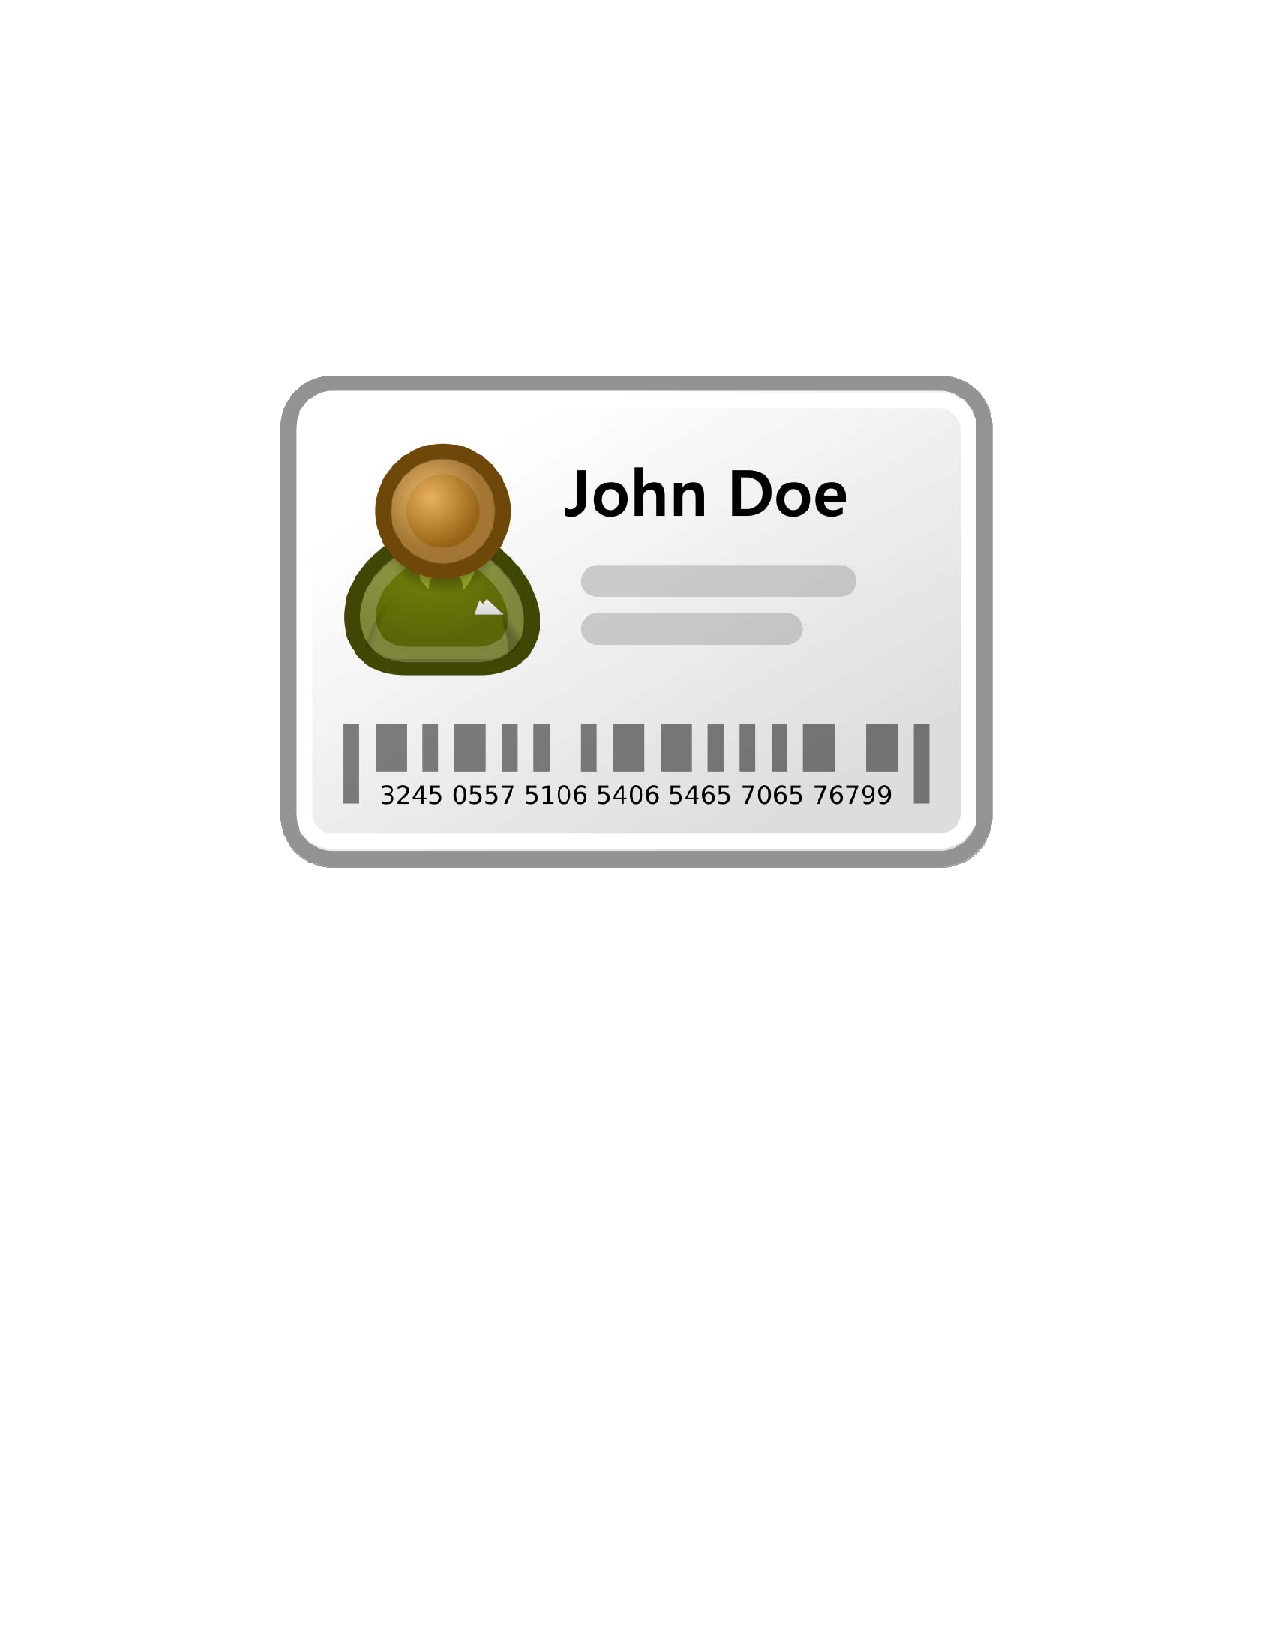
\includegraphics{id}
\end{center}
\cleardoublepage 

\part{Experiencia investigadora}

\chapter{Publicaciones científicas}
\cleardoublepage 

\section{Artículos en revistas}
\cleardoublepage 
%!TEX root = ../00_Documentacion_Completa/Acreditacion.tex

\newcommand{\revista}[4]{
\cleardoublepage
\vspace*{10cm}
\textsc{Artículo}:\\[5pt]
\uppercase{\textbf{#1}}\\
\bigskip

\textsc{Revista}: \uppercase{\textbf{#2}}\\

\textsc{Año de publicación}: \uppercase{\textbf{#3}}\\
\cleardoublepage
\includepdf[pages=-]{../04_EI_Revistas/#4}
}

\revista{Title}{Journal}{2018}{journal}%{1,2,3,4}


\section{Libros y capítulos de libros}
\cleardoublepage 
%!TEX root = ../00_Documentacion_Completa/Acreditacion.tex

\newcommand{\libro}[4]{
\vspace*{10cm}
\textsc{Libro}: \uppercase{\textbf{#1}}\\
\bigskip

\textsc{Capítulo}: \uppercase{\textbf{#2}}\\

\textsc{Año de publicación}: \uppercase{\textbf{#3}}\\
\cleardoublepage
\includepdf[pages=-]{../05_EI_Libros/#4}
}

\libro{Title}{Chapter}{2018}{book}


\cleardoublepage
\chapter{Participación en proyectos de investigación y/o en contratos de I+D}
\cleardoublepage 
%!TEX root = ../00_Documentacion_Completa/Acreditacion.tex


\includepdf[pages=-]{../06_EI_Participacion_proyectos/project_certificate}
\cleardoublepage


\cleardoublepage
\chapter{Patentes y otros resultados de la investigación, especialmente los que produzcan transferencia tecnológica al sector productivo}
\cleardoublepage
%!TEX root = ../00_Documentacion_Completa/Acreditacion.tex

\newcommand{\patente}[2]{
\cleardoublepage
\vspace*{10cm}
Título: 
\\[5pt]
\uppercase{\textbf{#1}}\\
\bigskip

\cleardoublepage
 
\includepdf[pages=-]{../07_EI_Patentes/#2}
}

\patente{Patent Title}{patent}



\cleardoublepage
\chapter{Tesis doctorales dirigidas}

\cleardoublepage
\chapter{Obras artísticas}

\cleardoublepage
\chapter{Contribuciones a congresos y conferencias científicas}
\cleardoublepage 
%!TEX root = ../00_Documentacion_Completa/Acreditacion.tex

\newcommand{\congreso}[4]{
\cleardoublepage
\vspace*{10cm}
\textsc{Artículo}:\\[5pt]
\uppercase{\textbf{#1}}\\
\bigskip

\textsc{Congreso/Conferencia}:\\[5pt]
\uppercase{\textbf{#2}}\\

\textsc{Año de publicación}: \uppercase{\textbf{#3}}\\

\cleardoublepage

\includepdf[pages=-]{../10_EI_Papers_y_congresos/#4}
}

\congreso{Title}{Conference}{2018}{conference}


\cleardoublepage
\chapter{Otros méritos relevantes de investigación}
\cleardoublepage 
%!TEX root = ../00_Documentacion_Completa/Acreditacion.tex

\cleardoublepage
\vspace*{10cm}
\uppercase{\textbf{JUSTIFICACIÓN DE ALGUNAS PARTICIPACIONES EN ...}}
\cleardoublepage


\includepdf[pages=-]{../15_EI_Otros_meritos_de_investigacion/others}

\cleardoublepage
\vspace*{10cm}
\textsc{Reconocimiento}:\\[5pt]
\uppercase{\textbf{BEST PRESENTATION AWARD}}\\

\bigskip

\textsc{Congreso/Conferencia}:\\[5pt]
\uppercase{\textbf{CONFERENCE}}\\

\textsc{Año}: \uppercase{\textbf{2018}}\\
\cleardoublepage


\includepdf[pages=-]{../15_EI_Otros_meritos_de_investigacion/others.pdf}








\part{Experiencia docente}

\cleardoublepage
\chapter{Puestos ocupados y docencia impartida}
\cleardoublepage 
%!TEX root = ../00_Documentacion_Completa/Acreditacion.tex

\section{Dedicación docente}
\cleardoublepage

\includepdf[pages=-]{../30_ED_Docencia_Impartida/certificate}

\section{Calidad de la actividad docente}
\cleardoublepage

\includepdf[pages=-]{../30_ED_Docencia_Impartida/certificate.pdf}


\cleardoublepage
\chapter{Cursos y seminarios impartidos orientados a la formación didactica universitaria}
\cleardoublepage 
%!TEX root = ../00_Documentacion_Completa/Acreditacion.tex

\cleardoublepage

\includepdf[pages=-]{../35_ED_Cursos_impartidos/course_certificate.pdf}


\cleardoublepage
\chapter{Cursos y seminarios recibidos y participación en congresos orientados a la formación didáctica universitaria}
\cleardoublepage 
%!TEX root = ../00_Documentacion_Completa/Acreditacion.tex

\cleardoublepage

\includepdf[pages=-]{../37_ED_Cursos_recibidos/course_certificate.pdf}


\cleardoublepage
\chapter{Elaboración del material docente y metodológico}
\cleardoublepage 

\cleardoublepage
\chapter{Participación en proyectos de innovación docente}
\cleardoublepage 

\cleardoublepage
\chapter{Otros méritos docentes relevantes}
\cleardoublepage 
%!TEX root = ../00_Documentacion_Completa/Acreditacion.tex

\cleardoublepage
\vspace*{10cm}
\uppercase{\textbf{Diplomas por ...}}\\

\cleardoublepage

\includepdf[pages=-]{../49_ED_Otros_meritos_docentes/other_certificates.pdf}

\cleardoublepage
\vspace*{10cm}
\uppercase{\textbf{Proyectos Fin de Carrera}}
\cleardoublepage

\includepdf[pages=-]{../49_ED_Otros_meritos_docentes/other_certificates.pdf}

\cleardoublepage
\vspace*{10cm}
\uppercase{\textbf{Trabajos Fin de Grado}}
\cleardoublepage

\includepdf[pages=-]{../49_ED_Otros_meritos_docentes/other_certificates.pdf}

\cleardoublepage
\vspace*{10cm}
\uppercase{\textbf{Trabajos Fin de Máster}}
\cleardoublepage

\includepdf[pages=-]{../49_ED_Otros_meritos_docentes/other_certificates.pdf}



\part{Formación académica}

\cleardoublepage 
\chapter{Titulación universitaria}
\cleardoublepage 
%!TEX root = ../00_Documentacion_Completa/Acreditacion.tex

\section{Título de ...}

\cleardoublepage

\includepdf[pages=-]{../50_FA_Titulo_Universitario/title_certificate}

\cleardoublepage
\section{Expediente académico}

\cleardoublepage

\includepdf[pages=-]{../50_FA_Titulo_Universitario/title_certificate}



\cleardoublepage 
\chapter{Doctorado}
\cleardoublepage 
%!TEX root = ../00_Documentacion_Completa/Acreditacion.tex

\cleardoublepage
\section{Título de doctor}

\cleardoublepage

\includepdf[pages=-]{../51_FA_Doctorado/title_certificate}

\cleardoublepage
\section{Tesis doctoral}

\cleardoublepage

\includepdf[pages=-]{../51_FA_Doctorado/title_certificate}

\cleardoublepage
\section{Resolución de la Secretaría de Estado de Universidades por las que se condece la mención de calidad y de excelencia al programa de doctorado ``PhD Program''}

\cleardoublepage

\includepdf[pages=-]{../51_FA_Doctorado/title_certificate}


\cleardoublepage 
\chapter{Otros títulos de postgrado}
\cleardoublepage 
%!TEX root = ../00_Documentacion_Completa/Acreditacion.tex

\newcommand{\titulopostgrado}[2]{
\cleardoublepage
\vspace*{10cm}
\textsc{Título}:\\[5pt]
\uppercase{\textbf{#1}}\\
\bigskip

\textsc{Universidad/Organismo responsable}:\\
\uppercase{\textbf{#2}}\\
\cleardoublepage
}

\titulopostgrado{Diploma/Certificado}{University}

\includepdf[pages=-]{../53_FA_Postgrado_u_otros/title_certificate}
% Include as many documents as required to justify
%
\includepdf[pages=-]{../53_FA_Postgrado_u_otros/title_certificate}






\cleardoublepage 
\chapter{Ayudas y becas}
\cleardoublepage 

\cleardoublepage 
\chapter{Estancias en centros españoles y extranjeros}
\cleardoublepage 
%!TEX root = ../00_Documentacion_Completa/Acreditacion.tex

\newcommand{\estancia}[2]{
\cleardoublepage 
\vspace*{10cm}
\textsc{Universidad/Organismo}:\\
\uppercase{\textbf{#1}}\\[5pt]
\bigskip
\textsc{Pais}:\\
\uppercase{\textbf{#2}}\\
\cleardoublepage
}

\estancia{University/Company}{Country}
% Include as many documents as required to justify

\includepdf[pages=-]{../55_FA_Estancia/stay_certificate}
\cleardoublepage

\includepdf[pages=-]{../55_FA_Estancia/stay_certificate}




\cleardoublepage 
\chapter{Cursos y seminarios de especialización}
\cleardoublepage 
%!TEX root = ../00_Documentacion_Completa/Acreditacion.tex


\includepdf[pages=-]{../60_FA_Cursos_especializacion/course_certificate.pdf}

\cleardoublepage

\includepdf[pages=-]{../60_FA_Cursos_especializacion/course_certificate.pdf}


\part{Experiencia profesional}
\cleardoublepage 

\cleardoublepage 
\chapter{Actividades de carácter profesional}
\cleardoublepage 
%!TEX root = ../00_Documentacion_Completa/Acreditacion.tex

\newcommand{\trabajo}[1]{
\cleardoublepage
\vspace*{10cm}
\textsc{Institución/Empresa}:\\[5pt]
\uppercase{\textbf{#1}}\\
\cleardoublepage
}

\trabajo{Company}

\includepdf[pages=-]{../70_EL_Actividades_Profesionales/employment_certificate}



\cleardoublepage 
\chapter{Otras actividades profesionales}
\cleardoublepage 
%!TEX root = ../00_Documentacion_Completa/Acreditacion.tex

% Free model

\cleardoublepage
\vspace*{10cm}
\textsc{Miembro de Comité}:\\[5pt]
\uppercase{\textbf{VOCAL DEL SUBCOMITE TECNICO DE NORMALIZACION ...}}\\
\cleardoublepage

\includepdf[pages=-]{../75_EL_Otras/others_certificate.pdf}

\cleardoublepage
\vspace*{10cm}
\uppercase{\textbf{Beca de colaboración en ...}}\\
\cleardoublepage

\includepdf[pages=-]{../75_EL_Otras/others_certificate.pdf}


\part{Otros méritos}
\cleardoublepage 
%!TEX root = ../00_Documentacion_Completa/Acreditacion.tex

\cleardoublepage
\vspace*{10cm}
\uppercase{\textbf{Curso de ...}}
\cleardoublepage

\includepdf[pages=-]{../80_Otros_meritos_relevantes/others_certificate}



\end{document}